\section{Resultate}\label{resultate}

Fits format, überprüfen wie viel es ausmacht. VOrgegriffen, lösung 0 \ref{resultate:loesung0} wird einmal im Fits und einmal alles als Binärdatei geschrieben.
figure
Die Resultate zeigen keinen signifikanten Unterschied des Speicherverbrauchs. Pro Feldlinie liegt der Unterschied bei einem Byte. Hochgerechnet sind es 1.2 KiBytes, welches das Fits-Format für sich beansprucht. Der Vorteil vom Fits Format ist, dass mögliche Byte-Ordering Probleme bereits abgefangen werden.

\subsection{Lösung 0, Angle-Subsampling} \label{resultate:loesung0}
Für die Lösung 0 soll nur das Subsampling, welches der JHelioviewer selbst durchführt, vor der Dateiübertragung durchgeführt werden. Dazu werden die Punkte in das kartesische Koordinatensystem umgerechnet und das angle-subsampling durchgeführt. anschliessend wird in das sphärische System rücktransformiert und schlussendlich die Datei mittels Rar komprimiert.
\begin{figure}[!htbp]
	\center
	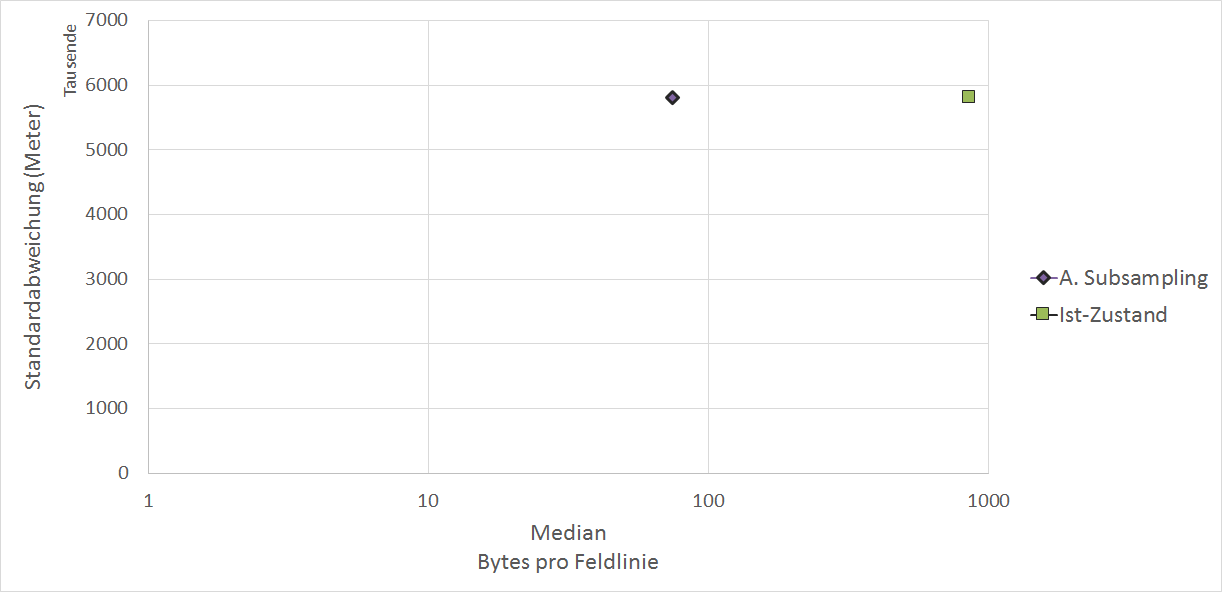
\includegraphics[width=0.8\textwidth,height=6cm,keepaspectratio]{./pictures/resultate/loesung0/loesung0_0.png}
	\caption{Vergleich der Lösung 0 zum Ist-Zustand.}
	\label{resultate:loesung0:loesung0_0}
\end{figure}
Wie im Diagramm \ref{resultate:loesung0:loesung0_0} erkennbar ist, verbraucht die Lösung 0 um grössenordnungen weniger Speicher. Rar scheint ebenfalls

\subsubsection{Variante PCA}
Durch die PCA könnte die Komprimierung weiter verbessert werden. Die unterschiedliche Orientierung der Feldlinien spielen keine Rolle mehr und die Chance ist höher, dass zwei Feldlinien ähnliche Punkte aufweisen. Dadurch könnte die Entropie-Kodierung eine bessere Kompression erzeugen.
Kartesische Koordinaten, Subsampling, 
figure
Leider nicht, es liegt zu einen an den Daten, welche zusätzlich gespeichert werden, 6 floats für das neuen koordinatenachsen und 3 floats für den Durchschnitt


\subsubsection{Artefakte}

\subsection{Lösung 1, Diskrete Kosinus Transformation}
Die Lösung 0 verbraucht bereits sehr viel weniger Speicher als der Ist-Zustand. Das Ziel ist nun eine bessere Kompression zu erreichen, indem die Feldlinien mit Kosinusfunktionen approximiert werden.
Momentan noch die ganze Kurve, deshalb ein Subsampling. Die Komplexität ist $O(n^2)$, was bei $600$ Punkten in einer Kurve zu erheblichen Rechenaufwand führt. Falls die Kompression 

Quantisierung

\subsubsection{DCT}
Nach dem Subsampling wird die Diskrete Kosinus Transformation ausgeführt. Die Koeffizienten werden anschliessend als 32Bit Integer abgespeichert.
Speicherung
Figure
Lösung leicht besser als die Lösung 0



\subsubsection{Angle-Subsampling mit DCT}
Nicht vielversprechend, da sehr hohe Varianz in den Daten, aber Angle-Subsampling wirft sehr viele Daten weg.
figure 
wie man sehen kann, klappt es nicht. Der Fehler schiesst in die Höhe

\subsubsection{Feldlinien Ableiten mit DCT}\label{resultate:dct:ableitung_dct}
ableitung
Speicherung
Weniger grosse Zahlen, dämpfung des DC-Koeffizienten. Dafür wird die Kurve immer Ungenauer.
figure vergleich Lösung1 und 1-1
Kann gut Quantisiert werden, es kann der Grossteil der DCT Komponenten auf 0 gesetzt werden. Es ist aber hier auch anzumerken, dass die VArianz hier stärker ins  Gewicht fällt, als bei purer DCT. Trotzdem ist sie besser und weist im selben Punkt die Hälfte vom maximalen Fehler auf. Bei $71$ Byte pro Linie liegt der maximale Fehler bei$70'000$ km anstatt bei $140'000$.
Die Speicherung könnte weiter verbessert werden, wenn die startpunkte diskretisiert werden, z.b. in diskrete sphärische Koordinaten. Rar scheint allgemein einfacher Integers komprimieren zu können.


\subsubsection{PCA mit DCT}
Idee: informationsgehalt anstatt auf alle 3 Kanäle verteilen, möglichst in einen konzentrieren, wie YCbCr in JPEG.

Figure vergleich mit purem dct
Resultat sehr ähnliches Verhalten wie ohne PCA

\subsubsection{Feldlinien Ableiten mit PCA und DCT}
Selbe Idee wie in \ref{resultate:dct:ableitung_dct}, nur 
figure Vergleich 1-1 und 1-4
Der Aufwand lohnt sich nicht, obwohl die PCA vielversprechend scheint. Feldlinien liegen ungefähr in einer Ebene. Dadurch kaum noch etwas im Z-kanal, fast alles 0.
DCTKoeffizientenvergleich
X Kanal allgemein grösser, aber y und z kanal tiefer. Schlussendlich scheint die PCA keinen signifikanten Vorteil zu bringen.


\subsubsection{Artefakte}
2D Feldlinie zeigen, normal und komprimiert
